% report.tex - HPC 714 Report
% Uncomment the below line for the double spaced, review copy
% \documentclass[draftclsnofoot,onecolumn,conference,11pt]{IEEEtran}
% Uncomment the below line for the two column, final copy
\documentclass[conference,twocolumn,10pt]{IEEEtran}

% Load packages for the report
\usepackage{cite}
\usepackage{array}
\usepackage{listings}
\usepackage[caption=false,font=normalsize,labelfont=sf,textfont=sf]{subfig}
\usepackage{url}
\usepackage{color}
\newcommand{\kostasnote}[1]{\textcolor{blue}{\bf #1}}
\newcommand{\bennote}[1]{\textcolor{magenta}{\bf #1}}
\lstset{language=SQL}

% Graphics and figures configuration
\usepackage[pdftex]{graphicx}
% declare the path(s) where your graphic files are
\graphicspath{{./figures/}}
% and their extensions so you won't have to specify these with
% every instance of \includegraphics
\DeclareGraphicsExtensions{.pdf,.jpeg,.png}

% Math package configuration
\usepackage{amsmath}
\interdisplaylinepenalty=2500

% correct bad hyphenation here
\hyphenation{op-tical net-works semi-conduc-tor}


\begin{document}

% report title
\title{A Data Management Solution for the\\ DNA App Store}


% author names and affiliations
\author{
    \IEEEauthorblockN{Konstantinos Xirogiannopoulos}
    \IEEEauthorblockA{\textit{University of Maryland}\\
    Department of Computer Science\\
    Email: kostasx@cs.umd.edu\\
    }

    \and
    \IEEEauthorblockN{Virinchi Srinivas}
    \IEEEauthorblockA{\textit{University of Maryland}\\
    Department of Computer Science\\
    Email: virinchi@cs.umd.edu\\
    }


}

% make the title area
\maketitle

% report abstract
\begin{abstract}
  There is starting to emerge widespread interest in fleshing out the vision of a DNA App Store; a platform for developing applications that aim at providing users with specific tidbits of insight about themselves based on their genotypes, in the context of the genotypes of multiple other individuals. In order to provide these insights efficiently and accurately, applications would need to leverage the rapidly growing data-pool of sequenced human genomes. Currently however, when it comes to genotype datasets in particular, data is stored in \textit{flat files} and has to be manually loaded in memory every time so it can be queried in an ad-hoc and sometimes suboptimal fashion. In this paper we propose a data management pipeline towards making this vision of a DNA app store not only possible but also highly versatile and scalable.

\end{abstract}

\section{Introduction}
In recent years, the fields of Computational Biology and Genomics have come a long way in developing technologies towards being able to sequence and analyze the human genome. As these technologies progress, so does our understanding of human genetics as well as the insight that can be gained from genomic analysis. More specifically, there has been significant interest in performing \textit{variant calling} towards identifying and later attempting ,through a series of analyses, to explain variations in the genomes of different individuals. A wide array of companies have also started to emerge, whose goal is to find common as well as differentiating traits between individuals based on their genotypes. This has sparked the vision for creating the \textit{DNA AppStore}; an infrastructure that leverages genomic sequencing datasets through a series of applications that would allow for specific types of queries against one's genome, that are usually answered using the pool of genomes collected from as many individuals as possible. These applications could range from simple retrieval and similarity queries, to complex analytics for one or more individuals at a time. Any application in such an environment would require efficient ``\textit{sequence once, query often}" data access to a large database filled with a variety of different datasets around the genomes of many individuals. For the purposes of this study, we assume that these queries are typically going to be queries on top of genotype data resulting from variant calling, and we focus on the efficient structured storage of this data.

\section{Current state of the DNA App Store}
The high-level philosophy behind the value of the DNA App Store is that ``\textit{The genome is an asset that you have for life, and you’ll keep going back to it.}"\cite{DNAappstore}.
% The vision of the DNA App Store is a centralized database that has genome data about millions of individuals; data that can be leveraged to answer specific questions about them. Any firm that buys the App will be able to access the sequenced DNA data. Further, customers might be able to control on who could access the data. Genomes contain information about health risks, physical traits and whom we are related to; DNA tests could lead to significant insights.
Companies that seem to be interested in the idea of the DNA App Store include Helix, 23andMe, Human Longevity (HLI), and  Ancestry. Ancestry and 23andMe are currently offering genome sequencing services for their users while HLI is mostly focused on analytics of already existent genome data. \textit{Helix} has plans to offer more competitive sequencing prices than either of the two aforementioned companies but is still at very early stages in development. Human Longevity is reportedly building the largest genotype and phenotype database in the world and is hoping to enable services like personalized disease treatment through leveraging these databases. \textit{23andMe} provides carrier status reports, ancestry, wellness and traits reports based on the sequenced genomes stored in their database. They are also the only company that currently exposes a REST API\footnote{\small \url{https://api.23andme.com/}} for developers to access a small portion of their datasets. Through their endpoints, developers are able to retrieve all SNP-chips for a specific user's genome or query SNPs in a particular location in the genome. Given a profile\_id, users can also query phenotype information, as well as information about the different haplogroups the individual belongs to. We unfortunately have no further insight on the back-end storage infrastructure any of these companies are utilizing in order to enable their services.

Some of the prevalent types of queries that seems to be of interest for the DNA App Store include queries regarding genomic similarity. One example would be ``How similar am I genetically with X'' type queries. Albeit less optimal than ad-hoc solutions like GQT~\cite{layer2016efficient}, SQL does allow for queries like this while providing a rich platform for expressing custom user-defined aggregate functions and many different variations of the above query. One variation would be ``Show me the individuals that I have similarity $> 60\%$ with". Another type of query would be specific string querying on top of the genome; queries of the type ``Do I have the YY gene?" or if a specific character trait is correlated with a particular gene variant, users will want to ask ``Do I have this variant/mutation?" These types of queries are very natural for classic databases and are some of the queries we expect to be more commonplace in a system like the DNA App Store. These queries would essentially comprise \textit{independent apps} in the App Store and developers have the flexibility of either assigning the computational task to the database, or simply retrieving the data they require for the computation, and execute their own analysis on top of it.

\section{Related Work}
There has been a body of recent work that explores using \textit{database systems} in order to properly organize and efficiently query genomics data.

\begin{figure}[t]
    \centering
    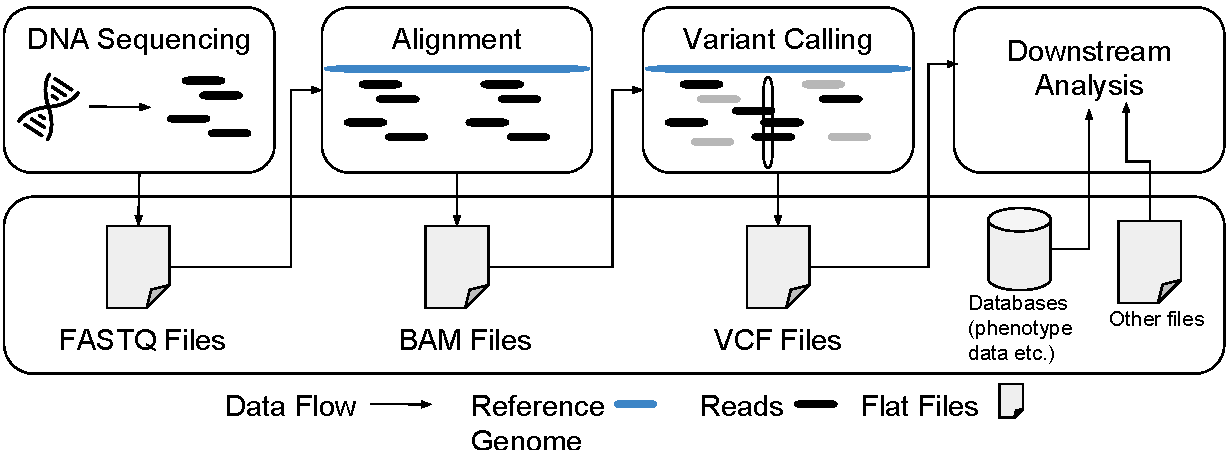
\includegraphics[width=0.50\textwidth]{current-pipeline}
    \caption{Current workflow using flat files (figure based on Figure 1 in \cite{dorok2015relational})}
    \label{fig:current}
    \vspace{-10pt}
\end{figure}

Dorok et al. \cite{dorok2015relational,dorok2015plants} proposes a \textit{base-centric} relational schema over the standard read-centric notion of storing raw sequence data, which avoids the on-the-fly cost of splitting reads when trying to search for specific bases. Their approach also leverages the inherent compression capabilities of column stores that do not require decompression at processing time. The fact that they are however using in-memory databases for this, although may increase query performance for some queries, will not scale to the volume of these datasets as cost of main memory is still quite far from reaching that of disk storage. Another work by Dorok et. al. \cite{dorok2014variant} utilizes user-defined aggregation functions in order to compute variant calls within the database on top of this schema using a combination of SQL and user-defined aggregation functions for implementing heuristics towards determining a genotype for each site in the requested range. This approach however significantly limits variant calling capabilities in the general case in that it renders a wide diversity of variant calling algorithms unusable, unless they are entirely re-implemented as user-defined functions on top of this schema.

The approach by R{\"o}hm et. al. \cite{rohm2009data} also towards storing raw sequence data into a Relational Database Management System (RDBMS) integrates genotyping by also utilizing user-defined aggregation functions however it chooses to store genome sequences as strings which require on-the-fly splitting via other user-defined functions. This work is mainly focused on trading off support for external tools for strict data modeling. The main purpose of this system is to store data from every stage of analysis including reads, alignments, meta-data about each of the reads, as well as the output of tertiary analysis (here they're storing consensus calling data). They are however using very small datasets to prove their points (in the order of a few GBs) and are not focusing on how this schema would scale. This line of work is in some ways however related to our goal of properly structuring genomics data towards higher availability and easier analysis however we focus specifically on genotype data that has resulted from variant calling.

There have also been a variety of systems \cite{bouffard2010damming, mitha2011snppy} that propose storing SNPs in structured relational databases \cite{codd1970relational} which allow for rich and efficient querying and analysis using SQL. The challenge with this architecture is the fact that it logically must include a single table containing every single variant that is observed for every individual as well as their homogeneity. This the space complexity of this single relation is of the order $v * i$ where $v$ is the number of unique variants and $i$ is the number of individuals in the dataset. Each work chooses to deal with this challenge differently; \cite{bouffard2010damming} partitions this table into a large set of smaller identical tables, without however specifically explaining whether or how these tables would be distributed across a cluster. SNPpy \cite{mitha2011snppy} on the other hand, endorses relational databases for their data validation mechanisms inherent in their data model as well as their ability to store multiple types of meta-data that can naturally be merged (joined) with the SNP data towards more complex analyses. Their results were however computed on very small simulated datasets (around 1.5 Million SNPs), so they did not encounter the aforementioned issue.

Moreover, there have been a few data warehouse solutions such as Atlas \cite{shah2005atlas} and BioWarehouse \cite{lee2006biowarehouse}; these solutions use disk-based relational databases but focus their efforts towards the issue of data integration across various different datasets relevant with bioinformatics and their solutions are not specifically optimized for genomic data.

More recently, the Genotype Query Tools (GQT) \cite{layer2016efficient} system has been proposed which enables fast queries over highly-compressed genotype data from VCF files. GQT however focuses specifically and is built in a way to efficiently support a specific subset of \textit{individual centric queries}. When it comes to variant-centric, or more complex queries such as searching for variants in specific chromosomal regions of the individuals, GQT breaks down. The reason is because GQT does not include any metadata associations with each variant they are storing in their index, making their approach very limited for more complex queries on top of genotype data.

There are also other open-source projects trying to deal with genomics data management, one of which is GenomicsDB~\cite{genomicsDB}, which is being developed by Intel. This project uses the TileDB \cite{tileDB} database (built for efficient sparse matrix/array storage) to store variant data in a 2D array, queried using a command line tool (similar to GQT) and returning results in a JSON format.

% Some of the companies that seem to be interested in the idea of the DNA App Store are Helix, 23andMe, Human Longevity, and  Ancestry. The idea of Helix is “sequence once, query often” which looks to collect DNA sample from any customer who buys the DNA app, sequence and analyze the customers’ genes, and then digitize the findings so that software developers can access it. Helix looks to create this digital hub of genomics in partnership with Illumina, Good Start Genetics and Duke University. Ancestry is another firm which aims at being able to trace one’s family story with a family tree. Once the tree is created the leaf node could be a hint to finding a match who could be your ancestor.

% Human Longevity (HLI) is building the largest genotype and phenotype database in the world to tackle and analyze some of the prevalent diseases like cancer, diabetes and obesity, heart and liver disease etc. They aim to leverage genomic and bioinformatic experience in diagnosing and treating the disease. They are sequencing complete genomes and plan to have the huge database of health records in the near future. Through database analysis, HLI is working towards developing personalized cancer vaccines based on an individual’s condition. The direction that HLI is approaching is to combine advances in genomics with personal health history to serve as a personalized approach in treatment.

% 23andMe provides carrier status reports, ancestry reports, wellness reports and traits reports based on the sequenced DNAs stored in their database. Their database has genes of approximately 1 million members acquired worldwide. 23andMe allows us to share the reports with friends and family. Further, 23andMe provides a REST API (https://api.23andme.com/) to be able to access the hundreds of thousands of SNPs. The API provides a very rich functionality.

% 23andMe API provides a wide variety of functionality which allows users to query for different types of information. The API allows access different types of information which can be categorized into 4 groups: User, Genetics, Phenotypes, and Ancestry. The return type for each GET method is a JSON object.

% User group endpoint queries consist of \texttt{GET /user, GET /names, GET, POST /profile\_picture}. \texttt{GET /1/user/}  gets the user id and a list of profile ids whether or not they are genotyped. \texttt{GET /1/names/profile\_id/} gets the first and last names for the user and user’s profiles. They also provide a possibility to get and post user’s profile picture.

% Genetics group of end point queries returns the base pairs for the user's profile for the given locations for the query \texttt{GET /1/genotypes/profile\_id/?locations=\&unfiltered}. \texttt{GET /1/genomes/profile\_id/?locations=\&unfiltered} returns the entire profile's genome as a packed string of base pairs.

% Phenotype based end point queries include \texttt{GET /1/phenotypes/profile\_id/phenotype\_id} retrieves the requested phenotype for the user’s profile while  \texttt{PUT /1/phenotypes/profile\_id/phenotype\_id} sets the requested phenotype data for the requested user profile.

% Further, the ancestry based end point queries consist of \texttt{GET/haplogroups/profle\_id} gets the maternal and paternal haplogroups as well as the terminal SNPs for the user’s profile.  \texttt{GET /1/ancestry/profile\_id/?threshold=…} provides ancestral breakdown for the user’s profile.  \texttt{GET /1/family\_members/?limit=x\&offset=y} returns all family members from the family tree based on the limit, offset parameters.  \texttt{GET /1/neanderthal/profile\_id} returns the estimated genome-wide proportion of Neanderthal ancestry for the user’s profile.


\section{Proposed Architecture}

A high level representation of the current pipeline architecture is depicted in Figure~\ref{fig:current}. Currently, genotype data is stored in flat files called VCF (Variant Call Format) files. These VCF files are then loaded into memory and analyzed using systems like \textit{samtools/bcftools}\footnote{\small \url{https://samtools.github.io/bcftools/bcftools.html}} for analysis. When it comes to variant-centric analysis, the performance of these tools starts becoming subpar due to the ever-expanding volume of data flowing into these flat files. This has caused the emergence ad-hoc solutions such as using compression schemes in order to be able to deal with the sheer volume of these datasets. These ad-hoc solutions however consequently limit the scope of analyses possible on top these datasets. In the context of a DNA App Store, various applications will require have access to a wide diversity of datasets, that they will undoubtably want to \textit{combine}, and apply extensive analysis on top of. The first step in that direction is bringing a higher degree of \textit{structure} to the genotype data that currently exists which will facilitate in analyzing it in a \textit{scalabile} and \textit{extensible} manner.

\begin{figure}[t]
    \centering
    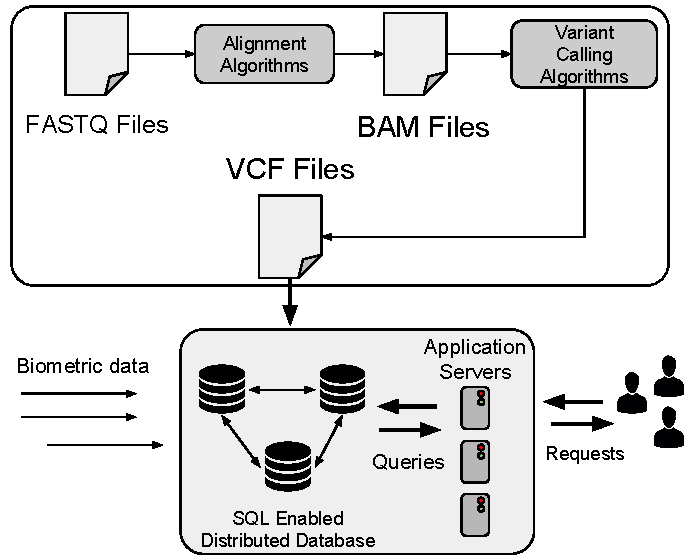
\includegraphics[width=0.35\textwidth]{proposed-pipeline}
    \caption{Our proposed architecture for the DNA App store}
    \label{fig:proposed}
    \vspace{-10pt}
\end{figure}

Our vision for how a data management system that would enable such rich analytics on top of genotype data is one that is optimized for the ``write-once, query-often" demands of the DNA App Store. The general idea is simple; apply ETL (Extract Transform and Load) over standard VCF files, insert them into a specific relational format dictated by a schema and then load it into a \textit{distributed database management system}.

Distributed databases are storage systems in which the data does not reside in a single machine. These systems provide replication across multiple nodes in a network which in turn offers both \textit{high availability} and \textit{fault-tolerance}. This means that the data store can handle a large amount of requests, even in situations when requests are hitting the same data at the same time, since most of the data will be replicated and will be able to be accessed from more than one machine at a time. The proposed schema is seen in Figure~\ref{fig:schema}. Genotype data has the unique characteristic that in order to enable complex analytics on top of it, one needs to store information about every single unique \textit{variant} for every \textit{individual} in one enormous logical relation; in our case that's the \texttt{Genotype} table. Using a distributed database, we can choose how to \textit{partition} this gigantic table in various ways across multiple machines.

We propose partitioning this \texttt{Genotype} table by \texttt{individual\_id} in a way such that all variants for a specific individual are stored \textit{in the same machine}. Advanced compression techniques already existent in most database systems will allow for further compressing the massive genotype table at every machine.
% This setup allows for rich analytics on top of variant datasets since it allows for also keeping meta-data.

\begin{figure}[t]
    \centering
    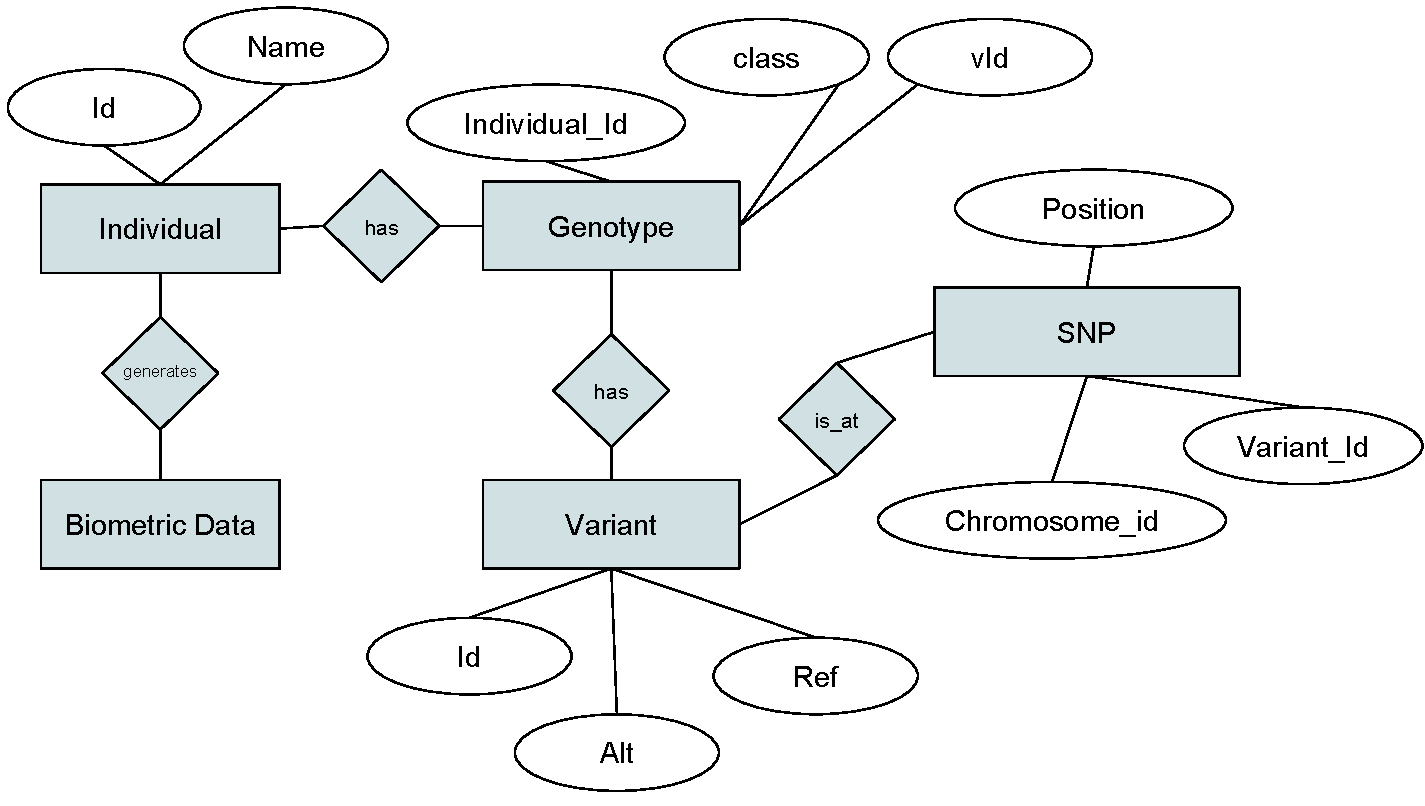
\includegraphics[width=0.45\textwidth]{schema}
    \caption{Our proposed schema for a distributed database for the DNA App Store}
    \label{fig:schema}
    % \vspace{-10pt}
\end{figure}

As mentioned, common queries would include finding the number of common genotypes between two individuals by using SQL; the following query will return how many variants a user named ``John Doe" has in common with Michael Jordan:
\begin{lstlisting}
With MJ as (Select G.class, G.vId
From Genotype G
Where G.Individual_id = (Select I.id from
Individuals I where name='Michael Jordan'))
Select Count(G.Vid) as common-variants
From Genotype G, MJ
Where G.Individual_Id = (Select I.id from
Individuals I where name='John Doe') and
G.vId = MJ.vId and G.class = MJ.class
\end{lstlisting}
Note that the similarity check does not necessarily have to be done in the database. Applications could simply query for the genotypes of these individuals and conduct their own analysis tailored to their purpose.

Because this is a write-once, read-many architecture, there are no issues of maintaining consistency in this context, since the genotype data is \textit{static}. Consistency would have been an issue if there were also a large number of incoming updates to the genome data, however in this case we have no updates to the genotypes that may interfere with the queries made by the applications since an individual’s variant data does not change once identified and inserted into the database.

Considering that there could potentially be as many as $100,000,000$ variants in the entire human genome, if we were to maintain the genotypes for as many as $1,000,000$ individuals, and store say $8$ bits per individual-variant pair (to account for multiple alleles, or complex structural variants), that would require $8*10^{14}$ bits, or $100$ Terabytes, before applying any standard compression techniques native in many database systems. We obviously don't have this volume of data available yet, but is steadily flowing in as more genomes are sequenced. Disk storage is also increasingly becoming more inexpensive, and it is currently not unusual for machines to have a few Terabytes of storage. By using a distributed architecture like the one proposed it is therefore apparent that a system like this is \textit{horizontally scalable}. Increase in data volume to extents much higher than this can be dealt with by simply throwing more machines at the problem.

% Therefore causality of updates is also not an issue in such a context due to the mostly static nature of genome data.

\section{Conclusion and Future Directions}
There are of course many more things to take into account like the actual rate at which queries are expected to hit this database, how we could incorporate biometric data into the equation, what interesting queries can be made by doing so and what potential problems arise in these cases. Moreover there could also arise problems regarding security and privacy as well as data ethics issues associated with the DNA App store as data anonymization is definitely non trivial and there may be interest in users’ genome data being completely anonymous but also that some of their phenotypes are concealed. It is difficult to predict whether these will be real issues or to estimate their magnitude in regards to the users as well as the infrastructure. Another future direction is incorporating more complex structural variants inside this database in ways that would enable combining these datasets with the rest of the data in the database (probably using SQL), towards potentially more insightful analytics.

We have proposed a database schema and architecture that would allow for structured queries of a large and extensible unified database system that we believe is a practical first step towards organizing the back-end for the vision of the DNA App store. We believe that allowing for SQL support over structured datasets would enable the realization of this vision as it would provide a standard, structured way of accessing and merging genomics data for complex analysis.

% conference papers do not normally have an appendix


% use section* for acknowledgment
% \section*{Acknowledgment}

% begin the references section.
\bibliographystyle{IEEEtran}
\bibliography{IEEEabrv,paper}



% that's all folks
\end{document}
